%%%%%%%%%%%%%%%%%%%%%%%%%%%%%%%%%%%%%%%%%
% Short Sectioned Assignment LaTeX Template Version 1.0 (5/5/12)
% This template has been downloaded from: http://www.LaTeXTemplates.com
% Original author:  Frits Wenneker (http://www.howtotex.com)
% License: CC BY-NC-SA 3.0 (http://creativecommons.org/licenses/by-nc-sa/3.0/)
%%%%%%%%%%%%%%%%%%%%%%%%%%%%%%%%%%%%%%%%%

%----------------------------------------------------------------------------------------
%	PACKAGES AND OTHER DOCUMENT CONFIGURATIONS
%----------------------------------------------------------------------------------------

\documentclass[paper=a4, fontsize=11pt]{scrartcl} % A4 paper and 11pt font size

% ---- Entrada y salida de texto -----

\usepackage[T1]{fontenc} % Use 8-bit encoding that has 256 glyphs
\usepackage[utf8]{inputenc}
%\usepackage{fourier} % Use the Adobe Utopia font for the document - comment this line to return to the LaTeX default

% ---- Idioma --------

\usepackage[spanish, es-tabla]{babel} % Selecciona el español para palabras introducidas automáticamente, p.ej. "septiembre" en la fecha y especifica que se use la palabra Tabla en vez de Cuadro

% ---- Otros paquetes ----

\usepackage{url} % ,href} %para incluir URLs e hipervínculos dentro del texto (aunque hay que instalar href)
\usepackage{amsmath,amsfonts,amsthm} % Math packages
%\usepackage{graphics,graphicx, floatrow} %para incluir imágenes y notas en las imágenes
\usepackage{graphics,graphicx, float} %para incluir imágenes y colocarlas

% Para hacer tablas comlejas
%\usepackage{multirow}
%\usepackage{threeparttable}

%\usepackage{sectsty} % Allows customizing section commands
%\allsectionsfont{\centering \normalfont\scshape} % Make all sections centered, the default font and small caps

\usepackage{fancyhdr} % Custom headers and footers
\pagestyle{fancyplain} % Makes all pages in the document conform to the custom headers and footers
\fancyhead{} % No page header - if you want one, create it in the same way as the footers below
\fancyfoot[L]{} % Empty left footer
\fancyfoot[C]{} % Empty center footer
\fancyfoot[R]{\thepage} % Page numbering for right footer
\renewcommand{\headrulewidth}{0pt} % Remove header underlines
\renewcommand{\footrulewidth}{0pt} % Remove footer underlines
\setlength{\headheight}{13.6pt} % Customize the height of the header

\numberwithin{equation}{section} % Number equations within sections (i.e. 1.1, 1.2, 2.1, 2.2 instead of 1, 2, 3, 4)
\numberwithin{figure}{section} % Number figures within sections (i.e. 1.1, 1.2, 2.1, 2.2 instead of 1, 2, 3, 4)
\numberwithin{table}{section} % Number tables within sections (i.e. 1.1, 1.2, 2.1, 2.2 instead of 1, 2, 3, 4)

\setlength\parindent{0pt} % Removes all indentation from paragraphs - comment this line for an assignment with lots of text

\newcommand{\horrule}[1]{\rule{\linewidth}{#1}} % Create horizontal rule command with 1 argument of height


%----------------------------------------------------------------------------------------
%	TÍTULO Y DATOS DEL ALUMNO
%----------------------------------------------------------------------------------------
\usepackage[sfdefault]{roboto}
\usepackage{sectsty}
\usepackage{hyperref}
\usepackage{listings}

\sectionfont{\fontsize{12}{15}\selectfont}
\title{
\normalfont \normalsize
\textsc{\textbf{Ingeniería de Servidores (2016-2017)} \\ Grado en Ingeniería Informática \\ Universidad de Granada} \\ [25pt] % Your university, school and/or department name(s)
\horrule{0.5pt} \\[0.4cm] % Thin top horizontal rule
\huge Memoria Práctica 2 \\ % The assignment title
\horrule{2pt} \\[0.5cm] % Thick bottom horizontal rule
}

\author{Sergio Cervilla Ortega} % Nombre y apellidos

\date{\normalsize\today} % Incluye la fecha actual

%----------------------------------------------------------------------------------------
% DOCUMENTO
%----------------------------------------------------------------------------------------

\begin{document}

\maketitle % Muestra el Título

\newpage %inserta un salto de página

\tableofcontents % para generar el índice de contenidos

\listoffigures


\newpage

%----------------------------------------------------------------------------------------
%	CUESTIÓN 1
%----------------------------------------------------------------------------------------

\section{a) Liste los argumentos de yum necesarios para instalar, buscar y eliminar paquetes.\newline b)¿Qué ha de hacer para que yum pueda tener acceso a internet en el PC del aula?\newline c) ¿Cómo añadimos un nuevo repositorio?}

\textbf{a)} Para instalar un paquete llamado \textit{package} deberemos de disponer de permisos root por tanto tenemos debemos de ejecutar los comandos con \textit{sudo} o ser superusuarios con \textit{sudo su}. Una vez aclarado esto, veamos como podemos resolver la cuestión:
\begin{itemize}
	\item Instalar: \begin{verbatim} sudo yum install -y package\end{verbatim}
	\item Buscar: \begin{verbatim} sudo yum search package\end{verbatim}
	\item Borrar: \begin{verbatim} sudo yum remove package\end{verbatim}
\end{itemize}

Hemos podido consultar estas órdenes la documentación oficial de yum \cite{man-yum}

\vspace{9mm}

\textbf{b) } Para poder hacer que yum disponga de Internet en el PC del aula debemos de configurar un proxy en el fichero situado en \textit{/etc/yum.conf} \cite{yum-proxy-conf}. Para ello deberemos de añadir una línea que contenga lo siguiente:\begin{verbatim}proxy=stargate.ugr.es:3128\end{verbatim} y cuyo formato genérico para añadir cualquier proxy es: \begin{verbatim}proxy=<url>:<port>\end{verbatim}

\vspace{9mm}

\textbf{c) } La forma recomendada para añadir un nuevo repositorio cuya url es \textit{repository-url} según RedHat es ejecutando el siguiente comando \begin{verbatim}sudo yum-config-manager --add-repo repository-url\end{verbatim} y no añadiendo el repositorio directamente a \textit{/etc/yum.conf} por motivos de seguridad \cite{yum-add-repo}.

%----------------------------------------------------------------------------------------
%	CUESTIÓN 2
%----------------------------------------------------------------------------------------
\section{a) Liste los argumentos de apt necesarios para instalar, buscar y eliminar paquetes.\newline b)¿Qué ha de hacer para que apt pueda tener acceso a internet en el PC del aula?\newline c) ¿Cómo añadimos un nuevo repositorio?}

\textbf{a)} Para instalar un paquete llamado \textit{package} deberemos de disponer de permisos root por tanto tenemos debemos de ejecutar los comandos con \textit{sudo} o ser superusuarios con \textit{sudo su}. Una vez aclarado esto, veamos como podemos resolver la cuestión:
\begin{itemize}
	\item Instalar: \begin{verbatim} sudo apt-get install package -y\end{verbatim}
	\item Buscar: \begin{verbatim} sudo apt-cache search package\end{verbatim}
	\item Borrar: \begin{verbatim} sudo apt-get remove/erase package\end{verbatim}
\end{itemize}

Para instalar o borrar paquetes hemos consultado el man de apt-get \cite{apt-get}. Para buscar un paquete hemos consultado el man de apt-cache \cite{apt-cache}.

\vspace{9mm}

\textbf{b) } Para poder hacer que apt disponga de Internet en el PC del aula debemos de configurar un proxy en el fichero situado en \textit{/etc/apt/apt.conf} \cite{apt-proxy-conf}. Para ello deberemos de añadir una línea que contenga lo siguiente:\begin{verbatim}Acquire::http::proxy "http://stargate.ugr.es:3128/";\end{verbatim} y cuyo formato genérico para añadir cualquier proxy es: \begin{verbatim}Acquire::http::proxy "http://<proxy>:<port>/";\end{verbatim}

\vspace{9mm}

\textbf{c) } Para añadir un nuevo repositorio debemos de editar el fichero \textit{/etc/apt/sources.list} añadiendo la siguiente línea: \begin{verbatim}deb http://download.webmin.com/download/repository sarge contrib\end{verbatim} En este ejemplo, estamos instalando \textit{Webmin}\cite{webmin} ya que lo necesitaremos más adelante y así podemos comprobar cómo se añade un repositorio firmado.\newline Después de haber añadido esta línea debemos de añadir la clave con la que está firmado el repositorio, para ello ejecutamos los siguientes comandos:
\begin{itemize}
	\item Nos situamos en el directorio /root: \begin{verbatim}cd /root\end{verbatim}
	\item Descargamos la clave: \begin{verbatim}sudo wget http://www.webmin.com/jcameron-key.asc\end{verbatim}
	\item Añadimos la clave a nuestras claves de confianza: \begin{verbatim}sudo apt-key add jcameron-key.asc\end{verbatim}
	\item Actualizamos la lista de repositorios: \begin{verbatim}sudo apt-get update\end{verbatim}
	\item Instalamos webim: \begin{verbatim}sudo apt-get install webmin\end{verbatim}
\end{itemize}
%----------------------------------------------------------------------------------------
%	CUESTIÓN 3
%----------------------------------------------------------------------------------------
\section{\textbf{a)} ¿Con qué comando puede abrir/cerrar un puerto usando
	ufw? Muestre un ejemplo de cómo lo ha hecho.\newline \textbf{b)} ¿Con qué comando puede
	abrir/cerrar un puerto usando firewall-cmd en CentOS? Muestre un ejemplo
	de cómo lo ha hecho.\newline \textbf{c)} Utilice el comando nmap para ver que,
	efectivamente, los puertos están accesibles.}

\textbf{a) } El firewall de Ubuntu se llama Uncomplicated Firewall \cite{ufw}. Para abrir un puerto debemos de utilizar la siguiente orden: \begin{verbatim}sudo ufw allow <port>/[tcp/udp]\end{verbatim} y para cerrarlo debemos de utilizar \begin{verbatim}sudo ufw deny <port>[tcp/udp]\end{verbatim} Si no especificamos tcp/udp, se aplican ambos protocolos al puerto. Algunos ejemplos de uso:\newpage


Primero comprobamos el estado actual de los puertos que tenemos abiertos con la orden \textit{uwf status}.

\begin{figure}[H]
	\centering
	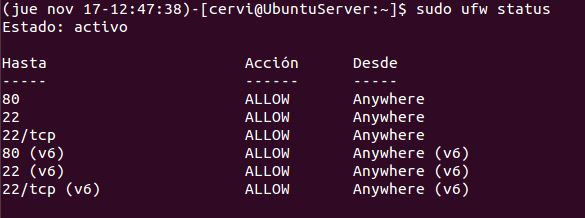
\includegraphics[scale=0.8]{ufw-status-1.jpg}
	\caption{Mostramos los puertos permitidos. \label{fig:figura1}}
\end{figure}

Ahora probamos a cerrar el puerto 22 con el protocolo tcp y comprobamos de nuevo el estado de los puertos
\begin{figure}[H]
	\centering
	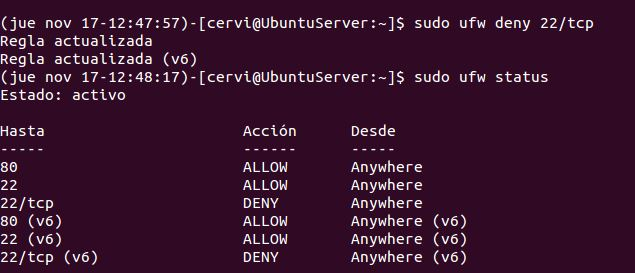
\includegraphics[scale=0.75]{ufw-deny-22tcp.jpg}
	\caption{Mostramos los puertos permitidos después de cerrar el 22 para tcp. \label{fig:figura2}}
\end{figure}

Para revertir este cambio tan solo tenemos que escribir la inversa de la orden anterior, es decir, si antes era \textit{ufw \textbf{deny} 22/tcp} ahora será \textit{ufw \textbf{allow} 22/tcp}

\begin{figure}[H]
	\centering
	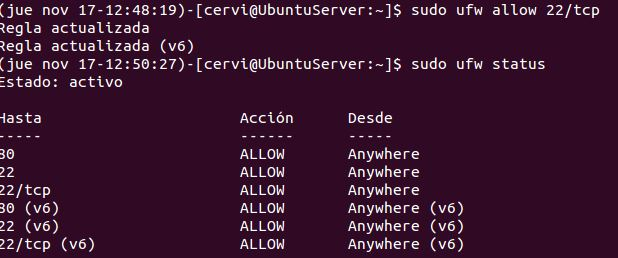
\includegraphics[scale=0.75]{ufw-allow.jpg}
	\caption{Mostramos los puertos permitidos después de cerrar el 22 para tcp. \label{fig:figura3}}
\end{figure}

Por último comprobamos que si no especificamos un protocolo, ufw lo cierra para ambos (tcp y udp).
\begin{figure}[H]
	\centering
	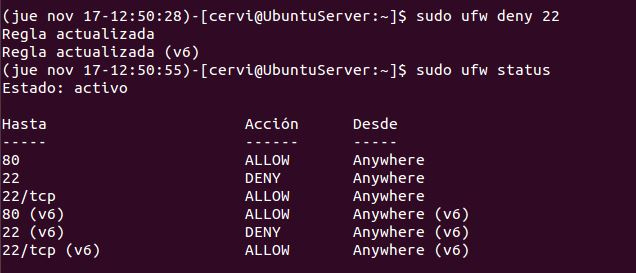
\includegraphics[scale=0.75]{ufw-deny-22.jpg}
	\caption{Mostramos los puertos permitidos después de cerrar el 22. \label{fig:figura4}}
\end{figure}

\textbf{b) } El firewall de CentOS se maneja con la orden firewall-cmd y para abrir un puerto debemos de utilizar la siguiente orden:
\begin{verbatim}sudo firewall-cmd --add-port=<port>/[tcp/udp]\end{verbatim}
y para cerrarlo debemos de utilizar
\begin{verbatim}sudo firewall-cmd --remove-port=<port>/[tcp/udp]\end{verbatim}

algunos ejemplos de uso:
\begin{figure}[H]
	\centering
	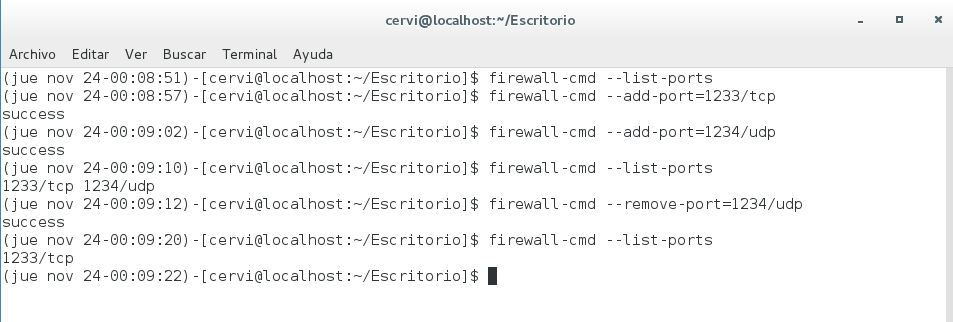
\includegraphics[scale=0.75]{firewall-cmd.jpg}
	\caption{Modificamos algunos puertos en CentOS. \label{fig:figura27}}
\end{figure}

\textbf{c) } Comprobamos con \textit{nmap localhost -p 22} que está abierto pero en caso de que nmap no pudiera acceder \underline{\textbf{no podríamos distinguir}} si es porque el servicio no está activo o porque el puerto está cerrado.

\begin{figure}[H]
	\centering
	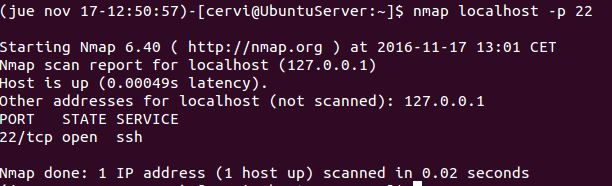
\includegraphics[scale=0.75]{nmap-accesible.jpg}
	\caption{Mostramos los puertos permitidos después de cerrar el 22. \label{fig:figura5}}
\end{figure}
%----------------------------------------------------------------------------------------
%	CUESTIÓN 4
%----------------------------------------------------------------------------------------
\section{¿Qué diferencia hay entre telnet y ssh?}
Aunque ambos comandos están pensados para conectar dos máquinas remotamente las diferencias saltan a la vista y esto es debido a la intención original de uso de cada comando. Para empezar, telnet\cite{telnet} fue ideado como una herramienta para comunicar ordenadores en una red privada en la cual no debíamos tener en cuenta ningún tipo de amenaza externa y por tanto el texto viaja sin ser encriptado de ninguna forma, viaja en texto plano. Sin embargo, ssh\cite{ssh} cifra el texto para evitar que con un simple programa de sniffing se pueda descubrir información potencialmente sensible. Además ssh ya fue diseñado con este propósito por lo que incluye un amplio abanico de opciones con las que usarse. Además el usuario que pretenda acceder debe de probar su autenticidad y que es quien dice ser a través de varios métodos, como puede ser el esquema de la llave pública y privada.
%----------------------------------------------------------------------------------------
%	CUESTIÓN 5
%----------------------------------------------------------------------------------------
\section{\textbf{a)} ¿Para qué sirve la opción -X?\newline \textbf{b)} Ejecute remotamente, es
	decir, desde la máquina anfitriona (si tiene Linux) o desde la otra máquina
	virtual, el comando gedit en una sesión abierta con ssh. ¿Qué ocurre?}

\textbf{a)} La opción -X de ssh sirve para habilitar el X11 forwarding. Esto significa que habilitamos
el servidor gráfico y por tanto podemos ejecutar aplicaciones con interfaz gráfica desde una máquina
remota. Por tanto, la aplicación se está ejecutando realmente en el servidor pero nosotros visualizamos
la interfaz gráfica en nuestra máquina con nuestro recursos.\newline
\textbf{b)} Primero establecemos una conexión ssh sin la opción -X e intentamos abrir un archivo con gedit:
\begin{figure}[H]
	\centering
	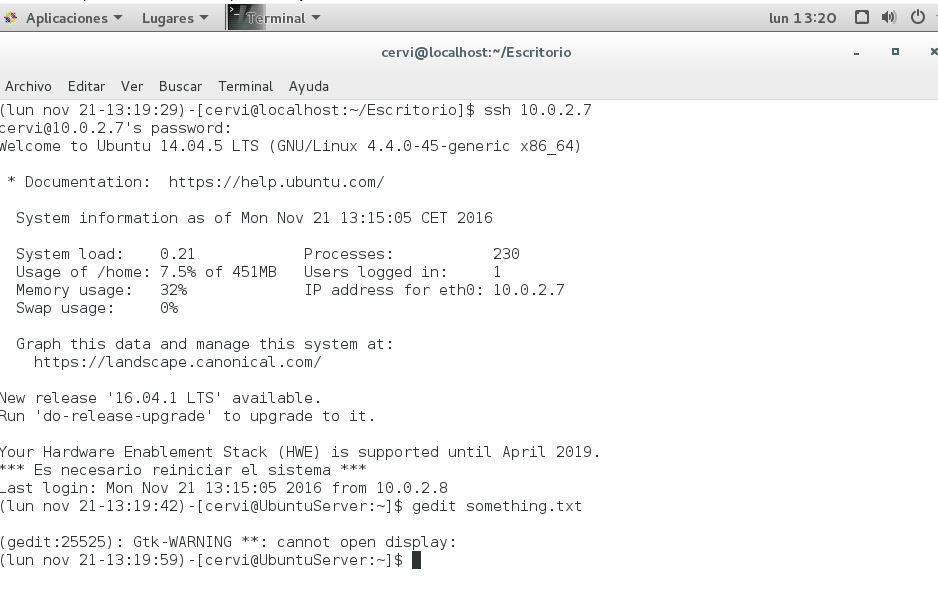
\includegraphics[scale=0.6]{ssh-no-x.jpg}
	\caption{Intento de ejecutar gedit sin la opción -X. \label{fig:figura10}}
\end{figure}
Como podemos imaginar, por defecto el X11 forwarding viene deshabilitado. Para poder utilizar el servidor gráfico añadimos la opción -X. Ahora intentamos abrir gedit y observamos que ocurre:
\begin{figure}[H]
	\centering
	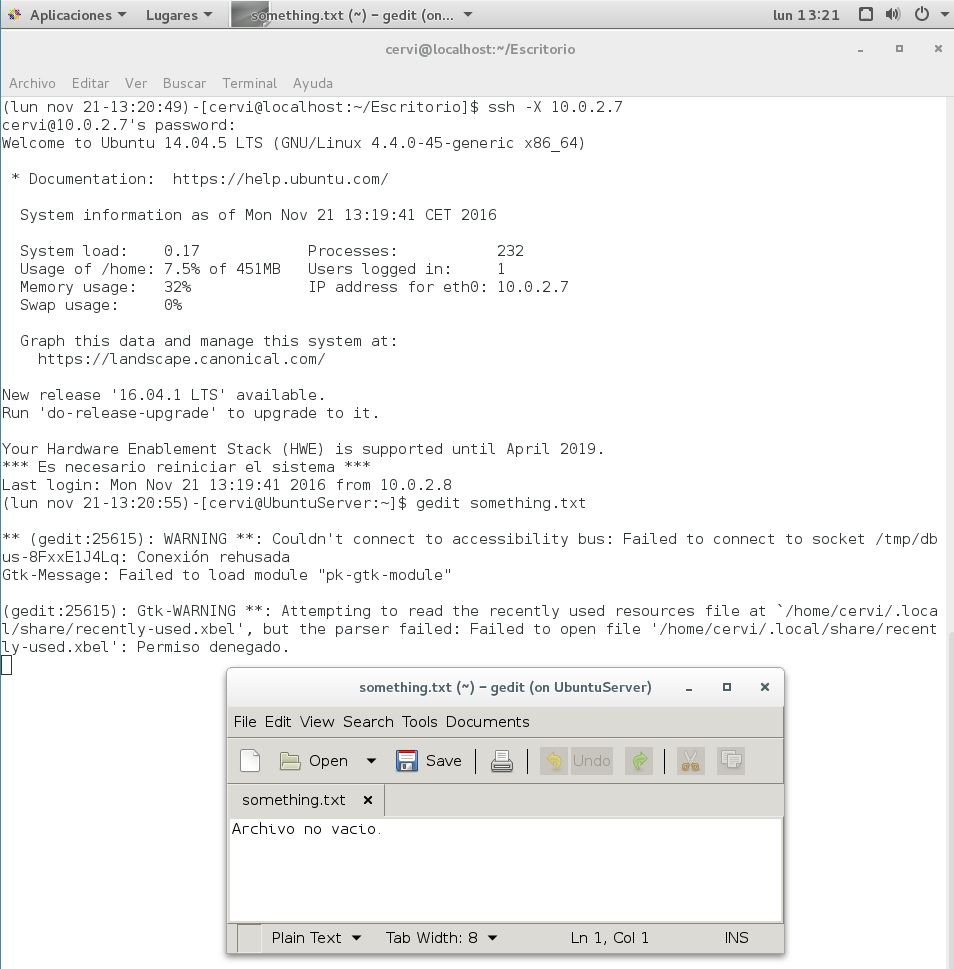
\includegraphics[scale=0.6]{ssh-X.jpg}
	\caption{Intento de ejecutar gedit con la opción -X. \label{fig:figura11}}
\end{figure}
En este caso si lo hemos podido ejecutar.
\newpage
%----------------------------------------------------------------------------------------
%	CUESTIÓN 6
%----------------------------------------------------------------------------------------
\section{Muestre la secuencia de comandos y las modificaciones a los archivos correspondientes para permitir acceder a la consola remota sin introducir la contraseña. Pruebe que funciona.}

Los pasos a seguir para conectarnos por shh utilizando el esquema de clave pública/privada es el siguiente:\newline
\begin{itemize}
	\item Generamos las claves con el algoritmo RSA de 4096 bits. Nos solicitará donde queremos que se guarde el archivo y una contraseña para protegerlo \newline
	\begin{figure}[H]
		\centering
		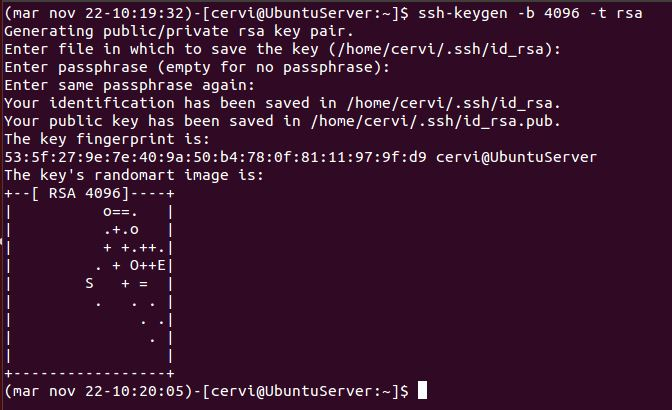
\includegraphics[scale=0.85]{ssh-keygen.jpg}
		\caption{Resultado de ejecutar ssh-keygen -b 4096 -t RSA. \label{fig:figura12}}
	\end{figure}
	\item Enviamos la clave pública a nuestro destinatario
		\begin{figure}[H]
		\centering
		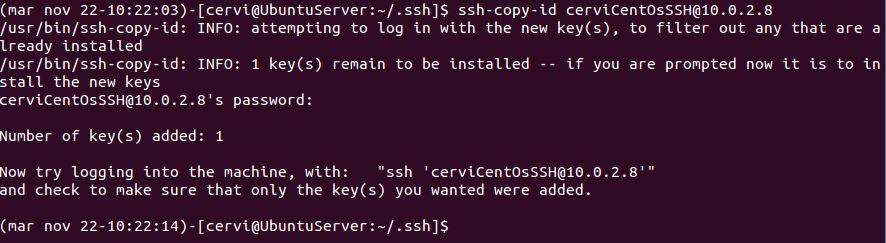
\includegraphics[scale=0.69]{ssh-copy-id.jpg}
		\caption{Resultado de ejecutar ssh-copy-id cerviCentOsSSH@10.0.2.8 \label{fig:figura13}}	\end{figure}
	\item Nos conectamos a la máquina y observamos como tan solo nos pide la contraseña de la clave
	que está guardada en local, pero no para realizar la conexión ssh.
	\begin{figure}[H]
		\centering
		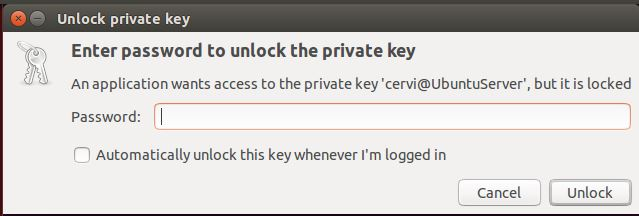
\includegraphics[scale=0.75]{private-key-auth.jpg}
		\caption{Solicitud de la contraseña para la clave privada. \label{fig:figura14}}
	\end{figure}
	\item Además, solo lo hace para la primera conexión de la sesión, es decir, que si nos quisiéramos conectar después de nuevo, no volvería a pedir la contraseña de la clave privada.
	\begin{figure}[H]
		\centering
		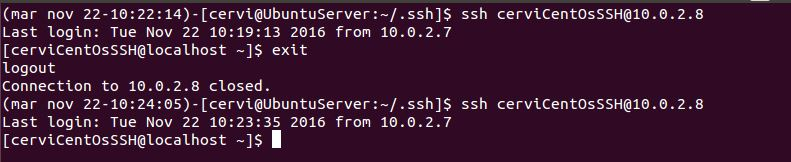
\includegraphics[scale=0.75]{ssh-no-pass.jpg}
		\caption{Conexión ssh sin contraseña. \label{fig:figura15}}
	\end{figure}
\end{itemize}
%----------------------------------------------------------------------------------------
%	CUESTIÓN 7
%----------------------------------------------------------------------------------------
\section{¿Qué archivo es el que contiene la configuración del servicio ssh? ¿Qué parámetro hay que modificar para evitar que el usuario root acceda? Cambie el puerto por defecto y compruebe que puede acceder.}

El archivo que contiene la configuración de ssh está situado en \textbf{/etc/ssh/sshd\textunderscore config}. Para evitar que el usuario root acceda debemos de cambiar la línea que contiene \begin{verbatim}
PermitRootLogin without-password\end{verbatim} por \begin{verbatim}
PermitRootLogin no\end{verbatim} Desactivar esta opción es bastante recomendable para la mayoría de los casos, pues que alguien se pueda hacer superusuario en nuestra máquina puede tener un efecto devastador en el sistema si tiene malas intenciones.\newline
Para cambiar el puerto por defecto debemos de modificar la línea que contiene \begin{verbatim}Port 22\end{verbatim} por \begin{verbatim}Port X\end{verbatim} donde X debe de ser un número de puerto válido y mayor que 1024, pues esos están reservados y podríamos inutilizar algún servicio de manera equívoca. Además deberemos de habilitad el tráfico en este puerto en el firewall, en el caso de Ubuntu con \begin{verbatim}ufw allow X\end{verbatim} y en CentOS con \begin{verbatim}firewall-cmd --add-port=X/tcp\end{verbatim}. Aquí tenemos una muestra de la conexión por ssh a través del puerto 51000
\begin{figure}[H]
	\centering
	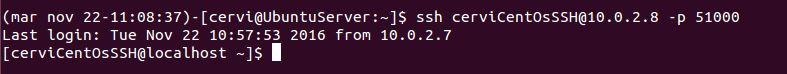
\includegraphics[scale=0.75]{ssh-51000.jpg}
	\caption{Conexión ssh en el puerto 51000. \label{fig:figura16}}
\end{figure}
%----------------------------------------------------------------------------------------
%	CUESTIÓN 8
%----------------------------------------------------------------------------------------
\section{Indique si es necesario reiniciar el servicio ¿Cómo se reinicia un servicio en Ubuntu? ¿y en CentOS? Muestre la secuencia de comandos para hacerlo.}

Sí, tendríamos que reiniciar el servicio pues los archivos de tipo \textbf{.conf} tan solo se leen una vez y es cuando se lanza el servicio. Por tanto, si lo modificamos después, debemos de reiniciar el servicio para que éste cargue el archivo ya modificado. En Ubuntu el servicio se reinicia de la siguiente manera: \begin{verbatim}/etc/init.d/ssh restart\end{verbatim} En CentOS la orden es la siguiente \begin{verbatim}service sshd restart\end{verbatim} o \begin{verbatim}/etc/init.d/sshd restart\end{verbatim}
%----------------------------------------------------------------------------------------
%	CUESTIÓN 9
%----------------------------------------------------------------------------------------
\section{Muestre los comandos que ha utilizado en Ubuntu Server y en CentOS (aunque en este último puede utilizar la GUI, en tal caso, realice capturas de pantalla). Compruebe que la instalación ha sido correcta.}
En el caso de Ubuntu es bastante sencillo pues con la orden \begin{verbatim}sudo apt-get install lamp-server^\end{verbatim} se instala todo automáticamente. Para comprobar que funciona tan solo tenemos que lanzar el servicio de apache2 con la orden \begin{verbatim}service apache2 start\end{verbatim} y accediendo en el navegador a \textbf{localhost} podemos comprobar que funciona.
\begin{figure}[H]
	\centering
	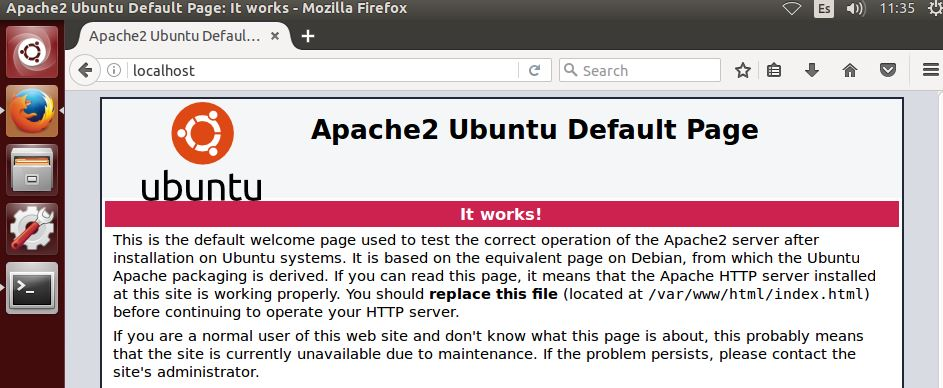
\includegraphics[scale=0.6]{apache2-ubuntu-works.jpg}
	\caption{Servicio Apache2 funcionando en Ubuntu. \label{fig:figura17}}
\end{figure}
\vspace{9mm}
En el caso de CentOS no existe un paquete que te instale todo y por tanto tenemos que proceder a instalar todos los paquetes uno a uno. Comenzaremos con Apache\cite{apache} y para ello utilizaremos la siguiente orden: \begin{verbatim}sudo yum install httpd\end{verbatim} y lo lanzamos con \begin{verbatim}sudo service httpd start\end{verbatim}
Acto seguido continuamos con MySQL\cite{mysql}. Deberemos de añadir el paquete de la comunidad para poder instalarlo, el proceso es el siguiente:
\begin{verbatim}wget http://repo.mysql.com/mysql-community-release-el7-5.noarch.rpm\end{verbatim}
\begin{verbatim}sudo rpm -ivh mysql-community-release-el7-5.noarch.rpm\end{verbatim}
\begin{verbatim}sudo yum update\end{verbatim}
Una vez tenemos todo lo necesario tan solo queda instalarlo ejecutando la siguiente orden
\begin{verbatim}sudo yum install mysql-community-server\end{verbatim} y lanzarlo \begin{verbatim}sudo service mysqld start\end{verbatim} Ahora procedemos a configurar MySQL ejecutando la orden \begin{verbatim}mysql_secure_installation\end{verbatim} y seguimos los sencillos pasos para configurar la contraseña y las opciones básicas como puede ser mantener la base de datos de test, permitir el acceso de superusuario remoto, etc.

Por último debemos de instalar PHP y para ello ejecutamos la siguiente orden \begin{verbatim}sudo \textbf{yum install php php-pear\end{verbatim}.

Ya solo queda reiniciar el servicio de apache2 y comprobar que todo está correcto:
\begin{figure}[H]
	\centering
	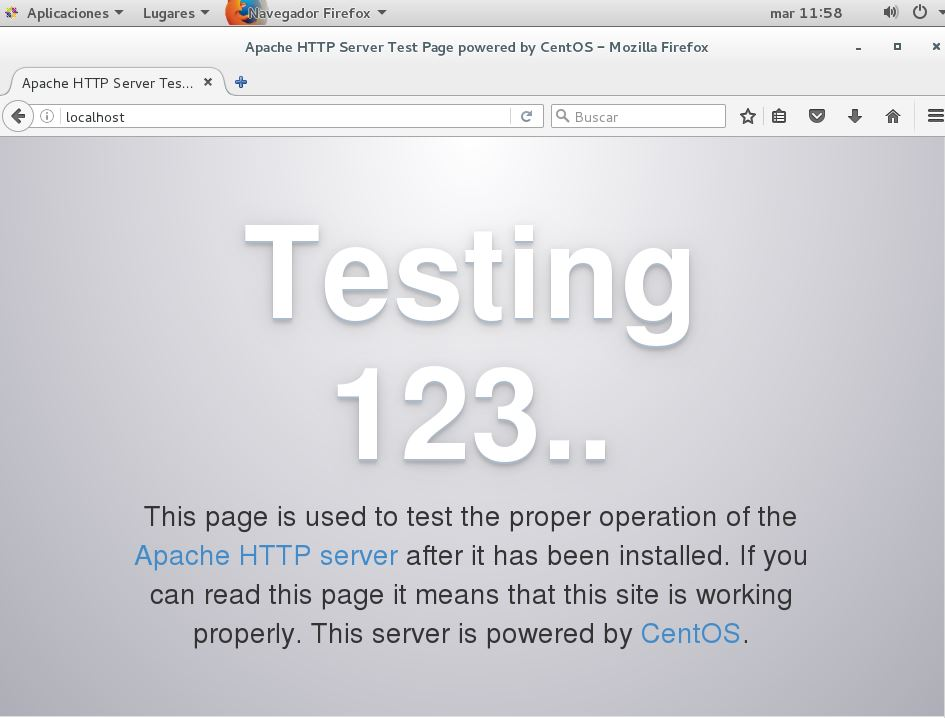
\includegraphics[scale=0.6]{apache2-centos-works.jpg}
	\caption{Servicio Apache2 funcionando en CentOS. \label{fig:figura18}}
\end{figure}
%----------------------------------------------------------------------------------------
%	CUESTIÓN 10
%----------------------------------------------------------------------------------------
\section{Realice la instalación de IIS usando GUI o PowerShell y compruebe que el servicio está funcionando accediendo a la MV a través de la anfitriona.}
Para realizar la instalación basta con seguir los simples pasos que nos indica el guión de la práctica. Para comprobar que funciona debemos de cambiar los ajustes de la máquina virtual. Actualmente tenemos el primer adaptador de red conectado a la red NAT y debemos de cambiar el segundo adaptador red por solo-anfitrión. Después de esto tenemos que ir a nuestro navegador en la máquina host y acceder al servidor mediante http://[ip-windows].
\begin{figure}[H]
	\centering
	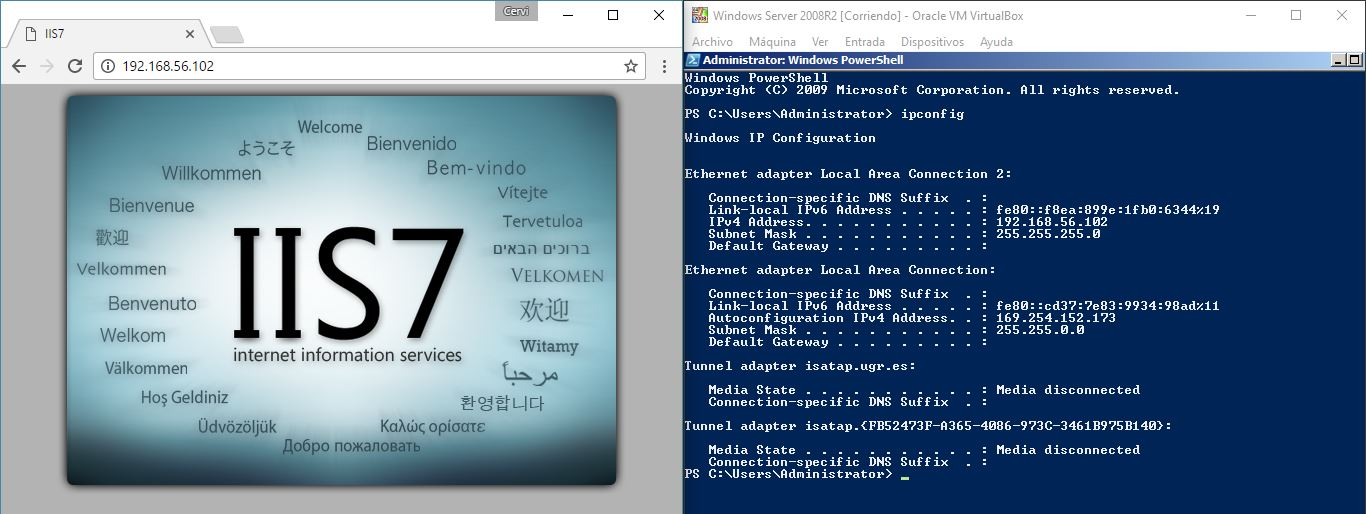
\includegraphics[scale=0.5]{iis.jpg}
	\caption{IIS funcinando. \label{fig:figura31}}
\end{figure}
%----------------------------------------------------------------------------------------
%	CUESTIÓN 11
%----------------------------------------------------------------------------------------
\section{Muestre un ejemplo de uso del comando patch.}
Imaginemos que somos el supervisor de un grupo de trabajo cuyo objetivo es entregar un programa a la comunidad y resulta que después de haber enviado el trabajo nos damos cuenta que han cometido algunos fallos ortográficos en la interfaz de nuestro programa como podemos observar en la siguiente imagen:
\begin{figure}[H]
	\centering
	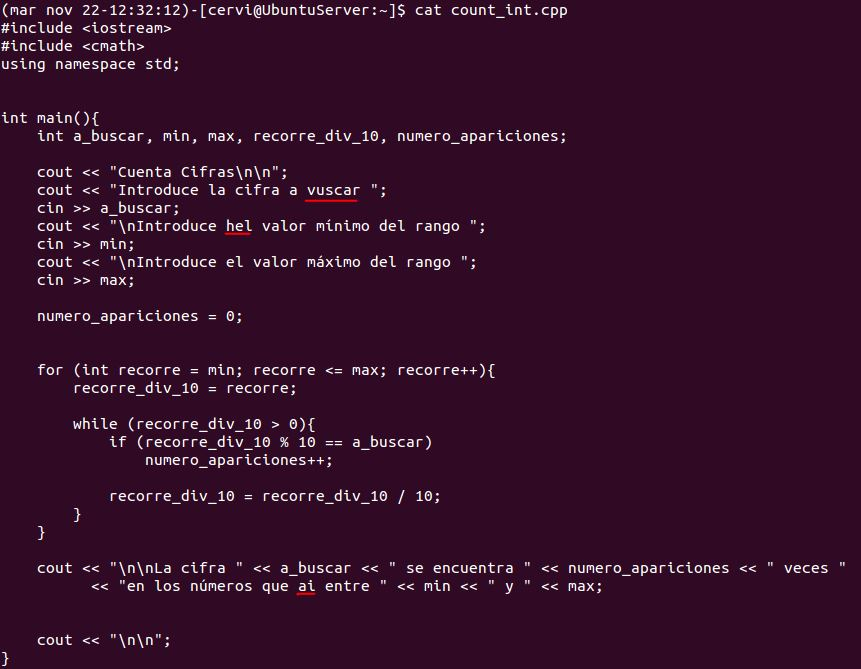
\includegraphics[scale=0.75]{cifras-mal.jpg}
	\caption{Programa con fallos. \label{fig:figura19}}
\end{figure}

Para solucionar este error podemos utilizar los dos comandos sugeridos, diff\cite{diff} y patch\cite{patch}. Si nos hemos dado cuenta de los errores y queremos solucionarlos con un parche  deberemos de seguir el siguiente procedimiento:
\begin{itemize}
	\item Cambiamos el nombre del archivo count\textunderscore cpp por count\textunderscore int\textunderscore err.cpp ya que no es correcto.
	\item Ejecutamos la siguiente orden para calcular los cambios del fichero correcto sobre el fichero erróneo y guardarlo en parche.patch\begin{verbatim}diff count_int_err.cpp count_int.cpp > parche.patch\end{verbatim}
	\vspace{9mm}
	\item Aplicamos el parche al archivo erróneo y comprobamos si se ha solucionado: \begin{verbatim} patch count_int_err.cpp parche.patch\end{verbatim}
	\begin{figure}[H]
		\centering
		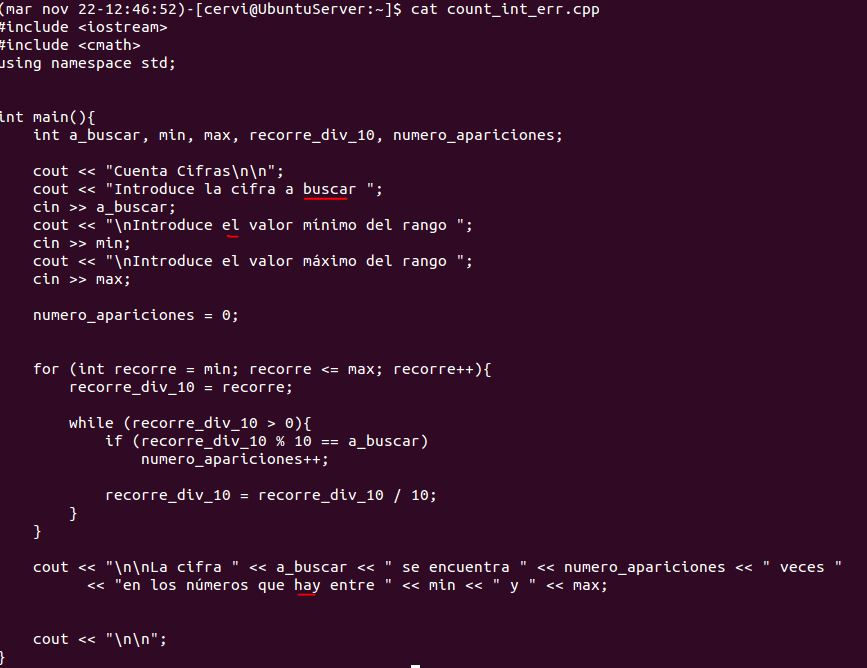
\includegraphics[scale=0.75]{cifras-bien.jpg}
		\caption{Programa corregido con patch y diff. \label{fig:figura20}}
	\end{figure}
\end{itemize}
%----------------------------------------------------------------------------------------
%	CUESTIÓN 12
%----------------------------------------------------------------------------------------
\section{Realice la instalación de esta aplicación y pruebe a modificar algún parámetro de algún servicio. Muestre las capturas de pantalla pertinentes así como el proceso de instalación.}
El proceso de instalación de \textbf{webmin} ya se encuentra en el apartado C del ejercicio 2.
Para acceder a Webmin debemos de escribir en el navegador https://ubuntuserver:10000 y nos pedirá que nos autentiquemos para lo que utilizaremos como usuario \textbf{cervi} y como contraseña la contraseña de root de nuestra sesión.
	\begin{figure}[H]
	\centering
	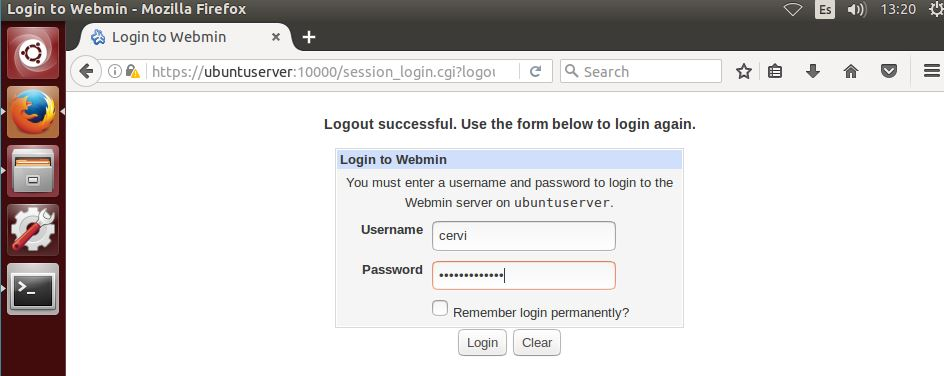
\includegraphics[scale=0.6]{webmin-login.jpg}
	\caption{Login para Webmin \label{fig:figura21}}
\end{figure}

Vamos a modificar algunas características del servicio ssh como pueden ser:
\begin{itemize}
	\item Reducir el número máximo de intentos fallidos por conexión a 3.
	\item Mostrar un mensaje personalizado antes de realizar la conexión.
	\item No permitimos que se autentiquen por contraseña ya que como hemos observado en ejercicios anteriores no es seguro. Por tanto se deben de autenticar con el esquema de llave pública y privada.
\end{itemize}
\begin{figure}[H]
	\centering
	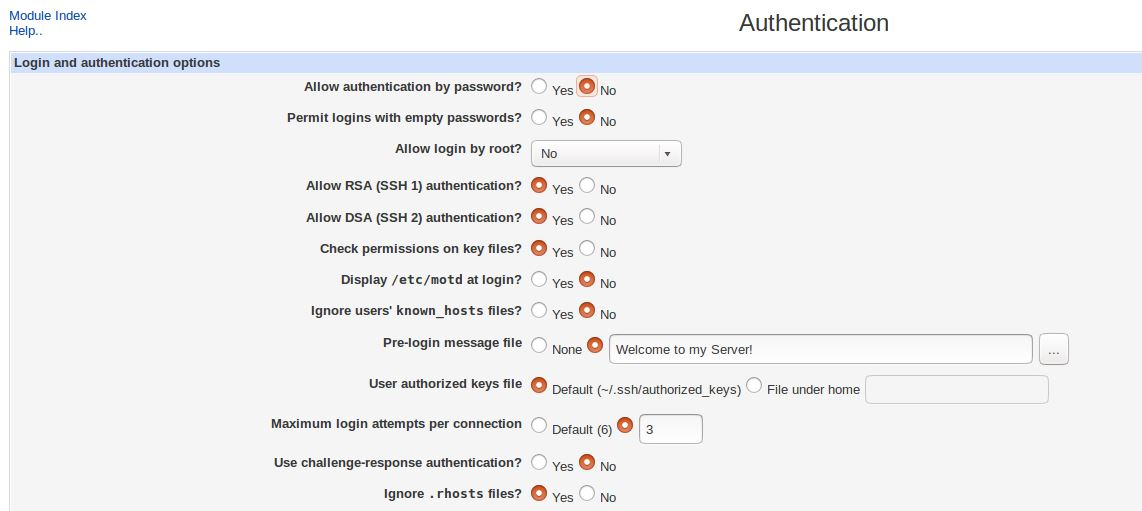
\includegraphics[scale=0.6]{webmin-change.jpg}
	\caption{Opciones modificadas del servicio de ssh. \label{fig:figura28}}
\end{figure}
%----------------------------------------------------------------------------------------
%	CUESTIÓN 13
%----------------------------------------------------------------------------------------
\section{Instale phpMyAdmin, indique cómo lo ha realizado y muestre algunas capturas de pantalla. Configure PHP para poder importar BDs de hasta 25MiB (en vez de los 8 MiB de límite por defecto). Indique cómo ha realizado el proceso y muestre capturas de pantalla.}
Para instalar phpMyAdmin\cite{phpmyadmin} tan solo tenemos que ejecutar la siguiente orden \begin{verbatim}sudo apt-get install phpmyadmin\end{verbatim} y para acceder debemos de poner en el navegador http://localhost/phpmyadmin despues de reiniciar el servicio. Para acceder ingresamos como usuario root y como contraseña la que hayamos establecido previamente.\newline
Para modificar el tamaño máximo a 25MiB debemos de acceder a la configuración de php que está situada en /etc/php5/apache2/php.ini y debemos de cambiar el tamaño en la siguiente línea. También deberemos de tener en cuenta que aunque aumentemos el tamaño máximo php tiene un time-out.
\begin{figure}[H]
	\centering
	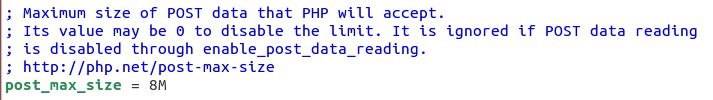
\includegraphics[scale=0.75]{php-max-size.jpg}
	\caption{Línea para modificar el tamaño máximo de las bases de datos a cargar. \label{fig:figura30}}
\end{figure}

%----------------------------------------------------------------------------------------
%	CUESTIÓN 14
%----------------------------------------------------------------------------------------
\section{Viste al menos una de las webs de los software mencionados	y pruebe las demos que ofrecen realizando capturas de pantalla y comentando qué está realizando.}

He visitado Direct Admin \cite{direct-admin} y vamos a utilizar la demo que ofrecen para ver que herramientas nos proporcionan. El problema es que no te deja hacer efectiva casi ninguna modificación porque la demo está muy restringida, por tanto, mostraré algunas cosas que podríamos hacer pero no puedo mostrar como quedaría el sistema después.

\begin{figure}[H]
	\centering
	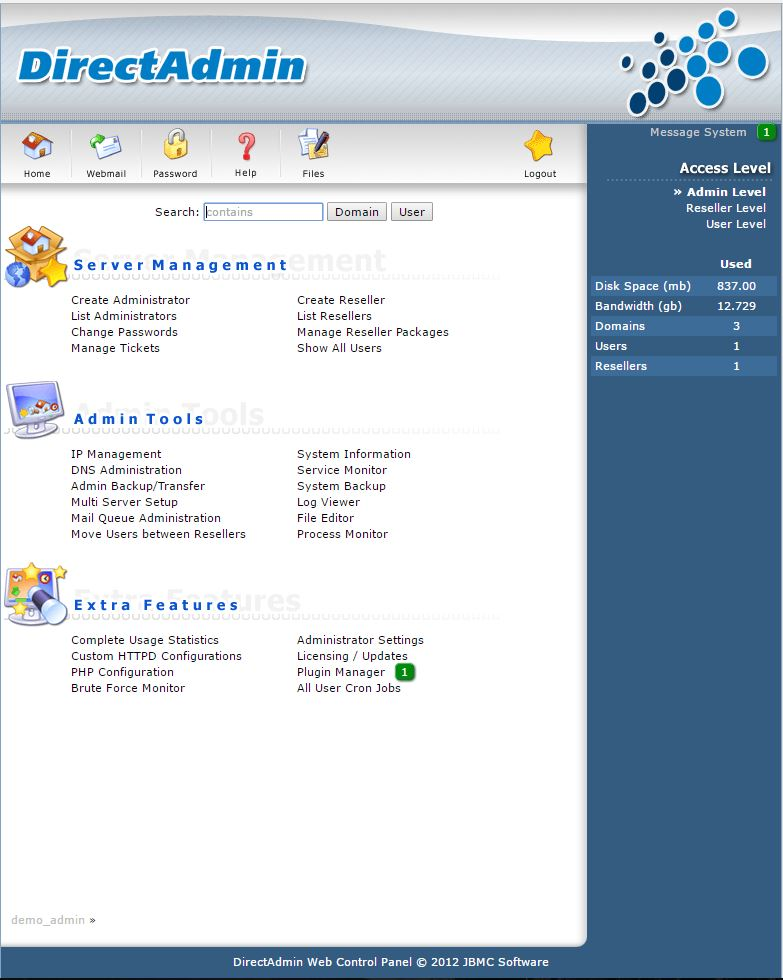
\includegraphics[scale=0.75]{direct-admin1.jpg}
	\caption{Panel principal de la demo de DirectAdmin. \label{fig:figura6}}
\end{figure}

Una vez hemos accedido podemos observar el panel de administrador en el que podremos realizar algunas pruebas como por ejemplo:\newline

\vspace{9mm}
\textbf{Crear un nuevo administrador:} Podemos crear un nuevo administrador tan solo rellenando los campos que nos solicitan.

\begin{figure}[H]
	\centering
	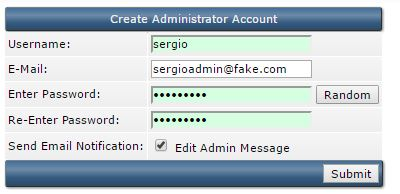
\includegraphics[scale=0.75]{create-admin.jpg}
	\caption{Datos para crear un nuevo administrador. \label{fig:figura7}}
\end{figure}
\vspace{9mm}
\textbf{Suspender la cuenta de un usuario:} Podemos suspender la cuenta de un usuario por varios motivos. En este caso lo haríamos por un uso excesivo del ancho de banda del servidor.

\begin{figure}[H]
	\centering
	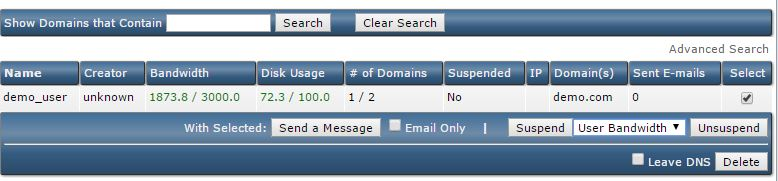
\includegraphics[scale=0.75]{ban-user.jpg}
	\caption{Panel de administración de usuarios. \label{fig:figura8}}
\end{figure}

\newpage

\textbf{Realizar una copia de seguridad del sistema:} Podemos realizar una copia de seguridad del sistema en la que podremos elegir los archivos y directorios que queremos guardar, transferirla por ftp/scp a otra máquina o incluso podemos utilizar cron para realizarla. Además de realizar copias de seguridad también podemos ver el log de la última copia.

\begin{figure}[H]
	\centering
	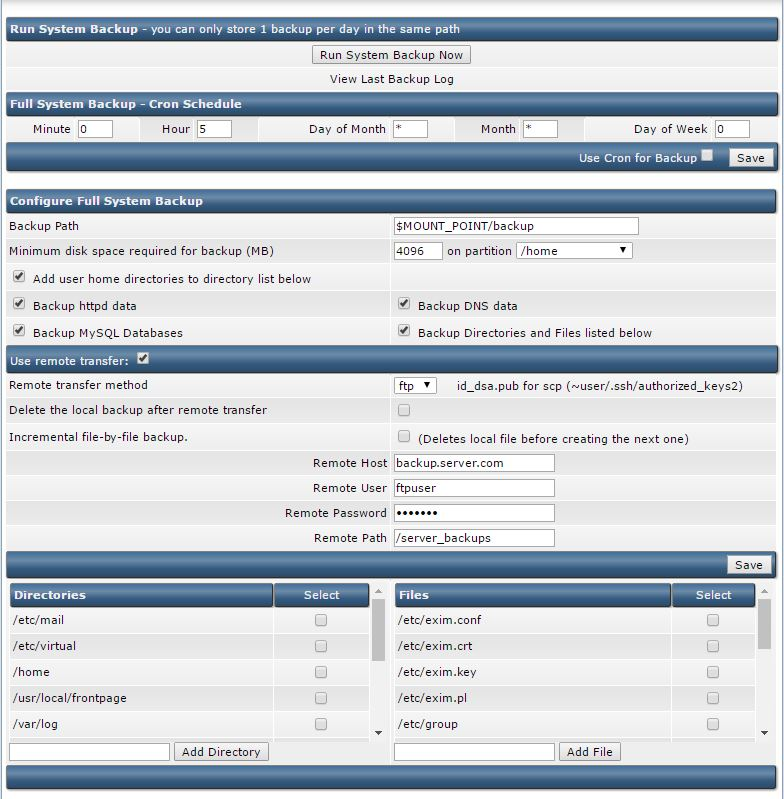
\includegraphics[scale=0.75]{backup.jpg}
	\caption{Panel de administración copias de seguridad. \label{fig:figura9}}
\end{figure}

%----------------------------------------------------------------------------------------
%	CUESTIÓN 15
%----------------------------------------------------------------------------------------
\section{a) Ejecute los ejemplos de find, grep\newline b) Escriba el script que haga uso de sed para cambiar la configuración de ssh y reiniciar el servicio.\newline c) Muestre un ejemplo de uso para awk}

\textbf{a)} Primero analizamos la orden que utiliza grep\cite{grep}: \begin{verbatim}ps -Af | grep firefox\end{verbatim} Esta orden utiliza el comando ps\cite{ps} para mostrar los procesos que están activos en el momento de ejecutar la orden. Además le añade dos parámetros. La opción \textbf{-A} selecciona todos los procesos del sistema y la opción \textbf{-f} nos aporta un formato muy completo a la hora de visualizarlo. Si ha este comando le encadenamos la orden grep más la cadena \textit{firefox} solo va a mostrar el proceso de firefox activo con las opciones pasadas a ps. El resultado de esta orden en mi máquina fue la siguiente:
\begin{figure}[H]
	\centering
	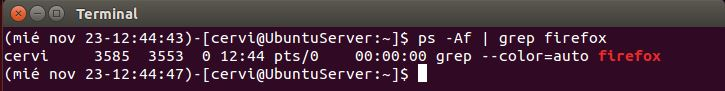
\includegraphics[scale=0.75]{ps-Af.jpg}
	\caption{Resultado de ejecutar \textbf{ps -Af | grep firefox}. \label{fig:figura22}}
\end{figure}

La segunda orden:  \begin{verbatim}find /home/alberto/docs -name '*pdf' -exec cp {} ~/PDFs \;\end{verbatim} Este comando lo tendremos que adaptar a nuestro caso pues la ruta especificada es válida para un usuario llamado alberto y que tenga la carpeta docs y PDFs. Voy a realizar unas pequeñas modificaciones para que funcione en mi caso y la orden queda tal que
\begin{verbatim}find ~/docs -name '*.pdf' -exec cp '{}' ~/PDFs \;\end{verbatim}

He creado ambas carpetas, docs y PDFs, para poder ilustrar el ejemplo. La orden find\cite{find} con el parámetro -name filtra todos los archivos por la cadena de texto siguiente que en este caso es que tengan extensión pdf (no que acabe en pdf, pues un archivo puede llamarse soyunpdf y tener extensión .txt). Después se le ordena con -exec que a los archivos que pasen ese filtro se copien en el directorio que cuelga del home del usuario llamado PDFs. Este ha sido el resultado:
\begin{figure}[H]
	\centering
	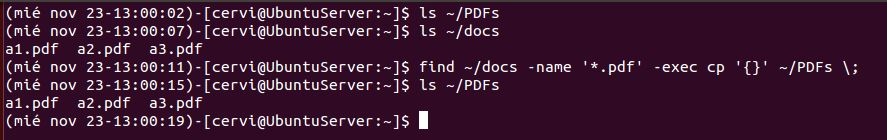
\includegraphics[scale=0.7]{find-pdfs.jpg}
	\caption{Resultado de ejecutar \textbf{find \textasciitilde/docs -name '*.pdf' -exec cp ' \textbraceleft \textbraceright ' \textasciitilde/PDFs \textbackslash;}. \label{fig:figura23}}
\end{figure}

\textbf{b)} Para este apartado vamos a hacer un script en el que sed\cite{sed} se encargue de procesar el fichero \textbf{sshd-config} para sustituir el puerto por defecto por el que le pasemos por parámetro al script. También he tenido en cuenta en el script que el puerto debe de ser mayor que 1024 para evitar posibles errores con otros conflictos. El script es el siguiente:
\begin{lstlisting}[language=bash,caption={sed script}]
	#/bin/bash
	cd /etc/ssh
	new_port=$1
	if [ $new_port -gt 1024 ]; then
		sed -i "s/22/$new_port/1" sshd_config
		/etc/init.d/ssh restart

	else
		echo 'El puerto debe ser mayor que 1024.'
	fi
\end{lstlisting}
\vspace{9mm}
y una prueba de su ejecución:
\begin{figure}[H]
	\centering
	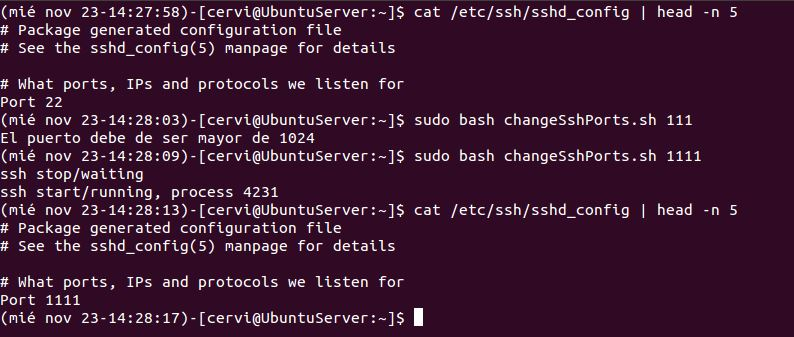
\includegraphics[scale=0.75]{sed-script.jpg}
	\caption{Resultado de la ejecución del script \textbf{changeSshPorts.sh}. \label{fig:figura24}}
\end{figure}

\textbf{b)} Para mostrar un ejemplo de awk he creado un script que busca en la configuración de ssh si existe algún puerto especificado y hace:
\begin{itemize}
	\item \textbf{Si existe:} Muestra el puerto por pantalla con un mensaje.
	\item \textbf{Si no existe:} Muestra un mensaje avisando de que no existe.
\end{itemize}
El script es el siguiente:
\begin{lstlisting}[language=bash,caption={sed script}]
	#/bin/bash
	cd /etc/ssh
	awk '/Port/{p=0;
		 if($1=="Port")
		   p=1;
		 if(p==1)
		   print "Puerto encontrado.",$2;
		 else if(p==0)
		   print "Puerto no encontrado.";
	}' sshd_config
\end{lstlisting}

prueba de su ejecución: 
\begin{figure}[H]
	\centering
	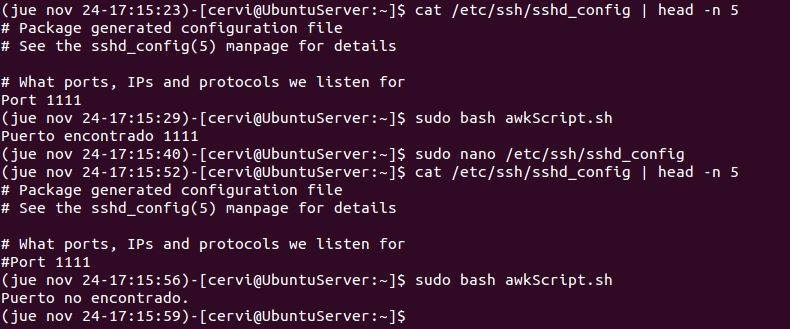
\includegraphics[scale=0.75]{awk-script.jpg}
	\caption{Resultado de la ejecución del script \textbf{awkSearch.sh}. \label{fig:figura32}}
\end{figure}
\newpage
%----------------------------------------------------------------------------------------
%	CUESTIÓN 16
%----------------------------------------------------------------------------------------
\section{Escriba el script para cambiar el acceso a ssh usando PHP o Python.}
Como tan solo he podido aprender las nociones básicas de python, he conseguido hacer este programa pero es algo básico. Se encarga de
encontrar el puerto por defecto de ssh y cambiarlo por el que le hemos pasado como parámetro. El programa es el siguiente:

\begin{lstlisting}[language=python,caption={python search}]

		import fileinput
		import sys
		import subprocess
		
		config="/etc/ssh/sshd_config"
		old_port="Port 22"
		list1=sys.argv[1:]
		
		new_port="Port "+"".join(list1)
		
		for line in fileinput.input(config, inplace=1):
		    if old_port in line:
		        line = line.replace(old_port,new_port)
		    sys.stdout.write(line)
		subprocess.call("/etc/init.d/ssh restart")

\end{lstlisting}
y una prueba de su ejecución: 
\begin{figure}[H]
	\centering
	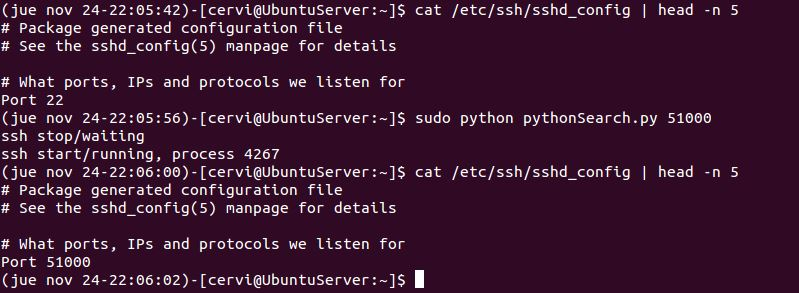
\includegraphics[scale=0.75]{python-search.jpg}
	\caption{Resultado de la ejecución de \textbf{pythonSearch.py}. \label{fig:figura29}}
\end{figure}

%----------------------------------------------------------------------------------------
%	CUESTIÓN 17
%----------------------------------------------------------------------------------------
\section{Abra una consola de Powershell y pruebe a parar un programa en ejecución (p.ej), realice capturas de pantalla y comente lo que muestra.}

Para parar un programa en ejecución tan solo tendremos que utilizar una de las tantas órdenes que nos ofrece PowerShell para lograr nuestra tarea. En este caso utilizaré \begin{verbatim}kill -proccessname\end{verbatim}\cite{powershell}

Antes de la ejecución del comando:
\begin{figure}[H]
	\centering
	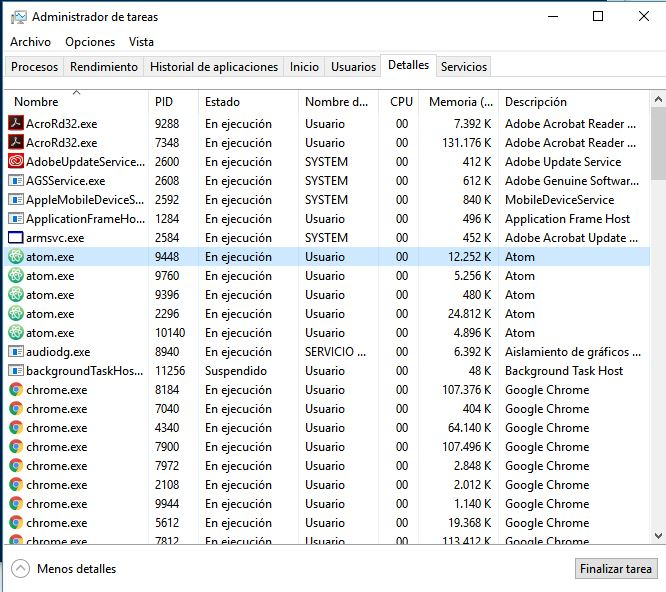
\includegraphics[scale=0.75]{before-kill.jpg}
	\caption{Procesos antes de ejecutar kill. \label{fig:figura25}}
\end{figure}
Después de la ejecución del comando:
\begin{figure}[H]
	\centering
	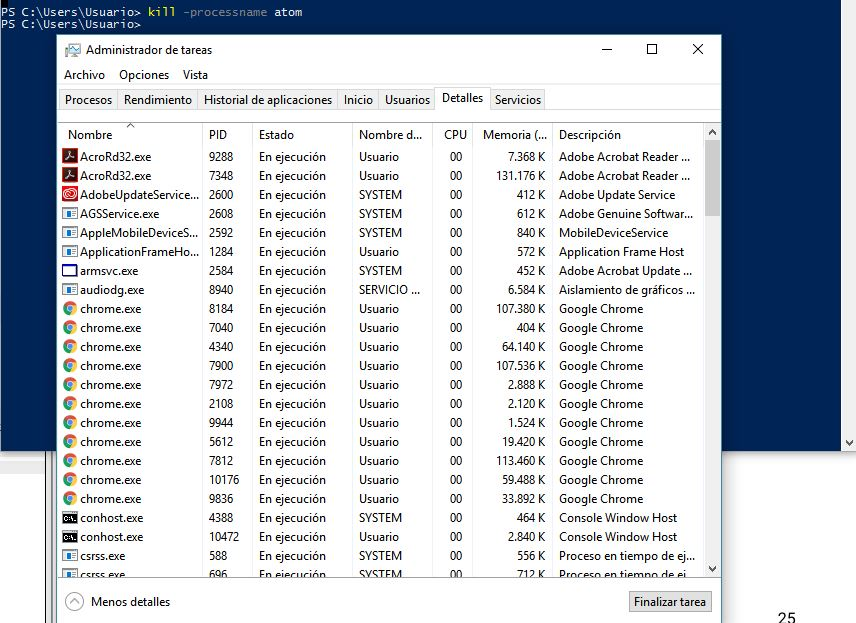
\includegraphics[scale=0.75]{after-kill.jpg}
	\caption{Procesos después de ejecutar kill. \label{fig:figura26}}
\end{figure}

\bibliography{citas} %archivo citas.bib que contiene las entradas
\bibliographystyle{plain} % hay varias formas de citar
\end{document}
